\documentclass[a4paper,10pt,twocolumn,oneside,x11names]{article}
\setlength{\columnsep}{10pt}  %兩欄模式的間距
\setlength{\columnseprule}{0pt}  %兩欄模式間格線粗細
\setlength{\headsep}{6pt}
\usepackage{amsthm}  %定義,例題
\usepackage{amssymb}
\usepackage[
    left=1cm,
    right=1cm,
    top=1.3cm,
    bottom=1cm,
]{geometry}
\usepackage{fontspec}  %設定字體
\usepackage{tikz}
\usepackage{color}
\usepackage{xcolor}
\usepackage{listings}  %顯示code用的
%\usepackage[Glenn]{fncychap}  %排版,頁面模板
\usepackage{fancyhdr}  %設定頁首頁尾
\usepackage{graphicx}  %Graphic
\usepackage{enumitem}
\usepackage{titlesec}
\usepackage{amsmath}
\usepackage{multicol}  %多欄模式
\usepackage[CheckSingle, CJKmath]{xeCJK}
% \usepackage{CJKulem}
%\usepackage[T1]{fontenc}
\titlespacing{\section}{0pt}{5pt}{1pt}
\titlespacing{\subsection}{0pt}{2pt}{0pt}
\usepackage{amsmath, courier, listings, fancyhdr, graphicx}
\usepackage{hyperref}
\hypersetup{
    colorlinks,
    citecolor=black,
    filecolor=black,
    linkcolor=black,
    urlcolor=black
}

%\renewcommand\listfigurename{圖目錄}
%\renewcommand\listtablename{表目錄} 

% ================================================ %

\setmainfont [ %主要字型
    UprightFont = *-Regular,
    BoldFont = *-Bold,
    ItalicFont = *-Italic
  ] {NotoSans}

\setmonofont [
    UprightFont = *-Regular
  ] {DMCA Sans Serif}

\setCJKmainfont{NotoSerifTC-Medium.otf} %中文字型
%\setmainfont{sourcecodepro}
\XeTeXlinebreaklocale "zh" %中文自動換行
\XeTeXlinebreakskip = 0pt plus 1pt %設定段落之間的距離
\setcounter{secnumdepth}{3} %目錄顯示第三層

% ================================================ %
\makeatletter
\lst@CCPutMacro\lst@ProcessOther {"2D}{\lst@ttfamily{-{}}{-{}}}
\@empty\z@\@empty
\makeatother
\lstset{
language=C++,
basicstyle=\footnotesize\ttfamily,
numberstyle=\tiny\color{gray},
stepnumber=1,
numbersep=5pt,
backgroundcolor=\color{white},
showspaces=false,
showstringspaces=false,
showtabs=false,
frame=false,
tabsize=4,
captionpos=b,
breaklines=true,
breakatwhitespace=false,
escapeinside={\%*}{*)},
morekeywords={*},
keywordstyle=\bfseries\color{Blue1},
commentstyle=\itshape\color{Red4},
stringstyle=\itshape\color{Green4},
numbers=left
}

% ================================================ %

\begin{document}
\renewcommand{\headrulewidth}{0.4pt}
\renewcommand{\contentsname}{Contents} 

\pagestyle{fancy}
\fancyfoot{}
\fancyhead[L]{NYCU Roselia}
\fancyhead[C]{Codebook}
\fancyhead[R]{\thepage}

% ================================================ %

{\scriptsize
\begin{multicols}{2}
\tableofcontents
\end{multicols}}

\section{Reminder}
\subsection{Bug List}
\begin{itemize}[nolistsep]
\item 沒開 long long
\item 陣列戳出界/開不夠大/ 開太大本地compile噴怪error
\item 傳之前先確定選對檔案
\item 寫好的函式忘記呼叫
\item 變數打錯
\item 0-base / 1-base
\item 忘記初始化
\item == 打成 =
\item <= 打成 <+
\item dp[i] 從 dp[i-1] 轉移時忘記特判 i > 0
\item std::sort 比較運算子寫成 < 或是讓 = 的情況為 true
\item 漏 case / 分case要好好想
\item 線段樹改值懶標初始值不能設為 0
\item DFS 的時候不小心覆寫到全域變數
\item 浮點數誤差
% \item unsigned int128
\item 多筆測資不能沒讀完直接 return
\item 記得刪 cerr
\end{itemize}

% \subsection{常見手法}
% \begin{itemize}[nolistsep]
% \item 對 OOO 排序
% \item 對值域做事
% \item 數值丟到數線上
% \item 數對 (a, b) $\Rightarrow$ 二維平面
% \item 區間問題:離線、雙指針、單調性
% \item 對答案的變動因素太多,可嘗試固定一種因素,並對它枚舉
% \item 把條件列出來分 case (ex. 三維偏序)
% \end{itemize}

\subsection{OwO}
\begin{itemize}[nolistsep]
% \item 注意變數範圍,誰特別大/特別小,作法 80\% 跟它有關。
% \item 題目「保證」某種性質作法 99\% 跟它有關。
% \item 寫下範測,釐清題目。
\item 可以構造複雜點的測資幫助思考
\item 真的卡太久請跳題
\item Enjoy The Contest!
\end{itemize}


\section{Basic}

% \subsection{Default}
% \lstinputlisting{code/basic/Default.txt}

\subsection{Vimrc}
\lstinputlisting{code/basic/vimrc}

\subsection{Runcpp.sh}
\lstinputlisting[language=sh]{code/basic/runcpp.sh}

%\subsection{Stress}
%\lstinputlisting[language=sh]{code/basic/stress.sh}

\subsection{PBDS}
\lstinputlisting{code/basic/PBDS.cpp}

\subsection{Random}
\lstinputlisting{code/basic/Random.cpp}

\subsection{pragma}
\lstinputlisting{code/basic/pragma.cpp}

\subsection{set map pq cmp}
\lstinputlisting{code/basic/cmp.cpp}

%\section{Python}
%\subsection{I/O}
%\lstinputlisting[language=Python]{code/python/PythonIO.txt}

%\subsection{Decimal}
%\lstinputlisting[language=Python]{code/python/PythonDecimal.txt}

\section{Data Structure}

\subsection{BIT}
\lstinputlisting{code/data-structure/BIT-wym.cpp}

\subsection{DSU}
\lstinputlisting{code/data-structure/DSU-wym.cpp}

\subsection{Segment Tree}
\lstinputlisting{code/data-structure/segtree-wym.cpp}

%\subsection{Merging on Seg-Tree}
%\lstinputlisting{code/data-structure/merging-on-seg-tree.cpp}

\subsection{Treap}
\lstinputlisting{code/data-structure/Treap.cpp}

\subsection{Persistent Treap}
\lstinputlisting{code/data-structure/persistent-treap.cpp}

\subsection{Li Chao Tree}
\lstinputlisting{code/data-structure/li-chao-tree.cpp}

\subsection{Sparse Table}
\lstinputlisting{code/data-structure/SparseTable.cpp}

\subsection{Time Segment Tree}
\lstinputlisting{code/data-structure/time-segtree.cpp}

\subsection{Dynamic Median}
\lstinputlisting{code/data-structure/Dynamic_Median.cpp}

\subsection{SOS DP}
\lstinputlisting{code/data-structure/SOS_DP.cpp}



%\section{DP}

%\subsection{Aliens}

%\lstinputlisting{code/dp/Aliens.cpp}

\section{Flow / Matching}

\subsection{Dinic}
\lstinputlisting{code/flow/Dinic.cpp}

%\subsection{ISAP}
%\lstinputlisting{code/flow/ISAP.txt}

\subsection{MCMF}
\lstinputlisting{code/flow/MCMF2.cpp}

\subsection{KM}
\lstinputlisting{code/flow/KM.cpp}

\subsection{Hopcroft-Karp}
\lstinputlisting{code/flow/HopcroftKarp.cpp}

\subsection{Blossom}
\lstinputlisting{code/flow/Blossom.cpp}

\subsection{Weighted Blossom}
\lstinputlisting{code/flow/WeightedBlossom.cpp}

\subsection{Cover / Independent Set}
\lstinputlisting{code/flow/CoverIndepend.txt}

\subsection{Hungarian Algorithm}
\lstinputlisting{code/flow/HungarianAlgorithm.cpp}


\section{Graph}

\subsection{Heavy-Light Decomposition}
\lstinputlisting{code/graph/HLD.cpp}

\subsection{Centroid Decomposition}
\lstinputlisting{code/graph/CentroidDecomposition.cpp}

\subsection{Bellman-Ford + SPFA}
\lstinputlisting{code/graph/BellmanFord + SPFA.cpp}

\subsection{BCC - AP}
\lstinputlisting{code/graph/BCC-AP.cpp}

\subsection{BCC - Bridge}
\lstinputlisting{code/graph/BCC-Bridge.cpp}

\subsection{SCC - Tarjan}
\lstinputlisting{code/graph/SCC-Tarjan.cpp}

\subsection{SCC - Kosaraju}
\lstinputlisting{code/graph/SCC-kosaraju.cpp}

\subsection{Eulerian Path - Undir}
\lstinputlisting{code/graph/EulerianPath-Undir.cpp}

\subsection{Eulerian Path - Dir}
\lstinputlisting{code/graph/EulerianPath-Dir.cpp}

\subsection{Hamilton Path}
\lstinputlisting{code/graph/HamiltonPath.cpp}

\subsection{Kth Shortest Path}
\lstinputlisting{code/graph/KSP.cpp}

\subsection{System of Difference Constraints}
\lstinputlisting{code/graph/DiffConstraints.cpp}
\begin{itemize}
	\item $x_u - x_v \le c \Rightarrow$ \texttt{add(v, u, c)}
	\item $x_u - x_v \ge c \Rightarrow$ \texttt{add(u, v, -c)}
	\item $x_u - x_v = c \Rightarrow$ \texttt{add(v, u, c), add(u, v -c)}
	\item $x_u \ge c \Rightarrow$ add super vertex $x_0 = 0$, then $x_u - x_0 \ge c$ $\Rightarrow$ \texttt{add(u, 0, -c)}
	\item Don't for get non-negative constraints for every variable if specified implicitly.
	\item Interval sum $\Rightarrow$ Use prefix sum to transform into differential constraints.  Don't for get $S_{i+1} - S_{i} \ge 0$ if $x_i$ needs to be non-negative.
	\item $\frac{x_u}{x_v} \le c \Rightarrow$ $\log{x_u} - \log{x_v} \le \log{c}$
\end{itemize}


\section{String}

\subsection{Aho Corasick}
\lstinputlisting{code/string/ACAutomaton2.cpp}

\subsection{KMP}
\lstinputlisting{code/string/KMP.cpp}

\subsection{Z Value}
\lstinputlisting{code/string/Zval.cpp}

\subsection{Manacher}
\lstinputlisting{code/string/Manacher.cpp}

\subsection{Suffix Array}
\lstinputlisting{code/string/SA-Optimized.cpp}

%\subsection{SA-IS}
%\lstinputlisting{code/string/SA-IS.cpp}

\subsection{Minimum Rotation}
\lstinputlisting{code/string/MinRotation.cpp}

\subsection{Lyndon Factorization}
\lstinputlisting{code/string/LyndonFactorization.cpp}

\subsection{Rolling Hash}
\lstinputlisting{code/string/RollingHash.cpp}

\subsection{Trie}
\lstinputlisting{code/string/Trie.cpp}

% \subsection{Suffix Array - Instruction}
% \lstinputlisting{code/string/SuffixArray-Instruction.cpp}

\section{Geometry}

\subsection{Basic Operations}
\lstinputlisting{code/geometry/GeometryDefault.cpp}

\subsection{Sort by Angle}
\lstinputlisting{code/geometry/SortByAngle.cpp}

\subsection{Intersection}
\lstinputlisting{code/geometry/LineIntersection.cpp}

\subsection{Polygon Area}
\lstinputlisting{code/geometry/PolygonArea.cpp}

\subsection{Convex Hull}
\lstinputlisting{code/geometry/ConvexHull.cpp}

\subsection{Point In Convex}
\lstinputlisting{code/geometry/PointInConvex.cpp}

\subsection{Point Segment Distance}
\lstinputlisting{code/geometry/PointSegmentDistance.cpp}

\subsection{Point in Polygon}
\lstinputlisting{code/geometry/PointInPoly.cpp}

\subsection{Minimum Euclidean Distance}
\lstinputlisting{code/geometry/MinEuclideanDist.cpp}

\subsection{Minkowski Sum}
\lstinputlisting{code/geometry/MinkowskiSum.cpp}

\subsection{Lower Concave Hull}
\lstinputlisting{code/geometry/LowerConcaveHull.cpp}


\subsection{Pick's Theorem}
Consider a polygon which vertices are all lattice points.

Let $i$ = number of points inside the polygon.

Let $b$ = number of points on the boundary of the polygon.

Then we have the following formula:

$$
Area = i + \frac{b}{2} - 1
$$

\subsection{Rotating SweepLine}
\lstinputlisting{code/geometry/rotating-sweepLine.cpp}

\subsection{Half Plane Intersection}
\lstinputlisting{code/geometry/half-plane-intersection.cpp}

\subsection{Minimum Enclosing Circle}
\lstinputlisting{code/geometry/MinEnclosingCircle.cpp}

\subsection{Union of Circles}
\lstinputlisting{code/geometry/UnionofCircles.cpp}

\subsection{Area Of Circle Polygon}
\lstinputlisting{code/geometry/area_of_cir_poly.cpp}

\subsection{3D Point}
\lstinputlisting{code/geometry/3DPoint.cpp}

\section{Number Theory}

\subsection{FFT}
\lstinputlisting{code/number-theory/FFT.cpp}

\subsection{Pollard's rho}
\lstinputlisting{code/number-theory/PollardRho-cpp.cpp}

\subsection{Miller Rabin}
\lstinputlisting{code/number-theory/MillerRabin.cpp}

\subsection{Fast Power}
{ \normalsize
Note: $a^n \equiv a^{(n \ mod \ (p-1))} (mod \ p)$
}

\subsection{Extend GCD}
\lstinputlisting{code/number-theory/ExtGCD.cpp}

\subsection{Mu + Phi}
\lstinputlisting{code/number-theory/Mu + Phi.cpp}

\subsection{Discrete Log}
\lstinputlisting{code/number-theory/Discrete-Log.cpp}

\subsection{sqrt mod}
\lstinputlisting{code/number-theory/sqrtmod.cpp}

\subsection{Primitive Root}
\lstinputlisting{code/number-theory/primitive_root.cpp}

\subsection{Other Formulas}
{\normalsize \begin{itemize}
    \item Inversion:\\ $aa^{-1} \equiv 1 \pmod{m}$. $a^{-1}$ exists iff $\gcd(a,m)=1$.
    
    \item Linear inversion:\\ $a^{-1} \equiv (m - \lfloor\frac{m}{a}\rfloor) \times (m \bmod a)^{-1} \pmod{m}$
    
    \item Fermat's little theorem:\\ $a^p \equiv a \pmod{p}$ if $p$ is prime.
    
    \item Euler function:\\ $\phi(n)=n \prod_{p|n} \frac{p-1}{p}$
    
    \item Euler theorem:\\ $a^{\phi(n)} \equiv 1 \pmod{n}$ if $\gcd(a,n) = 1$.
    
    \item Extended Euclidean algorithm:\\
    $ax+by=\gcd(a,b)=\gcd(b, a \bmod b)=\gcd(b, a-\lfloor\frac{a}{b}\rfloor b)=bx_1+(a-\lfloor\frac{a}{b}\rfloor b)y_1=ay_1+b(x_1-\lfloor\frac{a}{b}\rfloor y_1)$
    
    \item Divisor function:\\ $\sigma_x(n) = \sum_{d|n}d^x$. $n=\prod_{i=1}^r p_i^{a_i}$.\\ $\sigma_x(n)=\prod_{i=1}^r \frac{p_i^{(a_i+1)x}-1}{p_i^x-1}$ if $x \neq 0$. $\sigma_0(n)=\prod_{i=1}^r (a_i+1)$.
    
    \item Chinese remainder theorem (Coprime Moduli):\\ $x \equiv a_i \pmod{m_i}$.\\
        $M=\prod m_i$. $M_i=M/m_i$. $t_i=M_i^{-1}$.\\
        $x = kM + \sum a_i t_i M_i$, $k \in \mathbb{Z}$.
        
    \item Chinese remainder theorem:\\
    $x \equiv a_1 \pmod{m_1}, x \equiv a_2 \pmod{m_2} \Rightarrow x = m_1 p + a_1 = m_2 q + a_2 \Rightarrow m_1 p - m_2 q = a_2 - a_1$\\
    Solve for $(p, q)$ using ExtGCD.\\
    $x \equiv m_1 p + a_1 \equiv m_2 q + a_2 \pmod{lcm(m_1, m_2)}$
    
    \item Avoiding Overflow:
    $ca \mod cb = c(a \mod b)$
    
    \item Dirichlet Convolution: $(f * g)(n) = \sum_{d|n} f(n)g(n/d)$
    
    \item Important Multiplicative Functions + Proterties:
    \begin{enumerate}[nolistsep]
        \item $\epsilon(n) = [n = 1]$
        \item $1(n) = 1$
        \item $id(n) = n$
        \item $\mu(n) = 0$ if $n$ has squared prime factor
        \item $\mu(n) = (-1)^k$ if $n = p_1 p_2 \cdots p_k$
        \item $\epsilon = \mu * 1$
        \item $\phi = \mu * id$
        \item $[n=1] = \sum_{d|n} \mu(d)$
        \item $[gcd=1] = \sum_{d|gcd} \mu(d)$
    \end{enumerate}
    
    \item Möbius inversion:
    $f = g * 1 \Leftrightarrow g = f * \mu$
\end{itemize}}

\subsection{Polynomial}
\lstinputlisting{code/number-theory/Polynomial.txt}

\section{Linear Algebra}

\subsection{Gaussian-Jordan Elimination}
\lstinputlisting{code/linear-algebra/GaussElimination.cpp}

\subsection{Determinant}
{\normalsize
\noindent
\begin{enumerate}
\item Use GJ Elimination, if there's any row consists of only 0, then det = 0, otherwise det = product of diagonal elements.
\item Properties of det:
\begin{itemize}
    \item Transpose: Unchanged
    \item Row Operation 1 - Swap 2 rows: $-det$
    \item Row Operation 2 - $k \overrightarrow{r_i}$: $k \times det$
    \item Row Operation 3 - $k \overrightarrow{r_i}$ add to  $\overrightarrow{r_j}$: Unchaged
\end{itemize}
\end{enumerate}
}

\section{Combinatorics}

\subsection{Catalan Number}
$$
C_0=1, C_n=\sum_{i=0}^{n-1} C_i C_{n-1-i}, C_n=C_n^{2n}-C_{n-1}^{2n}
$$

\begin{center}
    \begin{tabular}{r|lllll}
        0 & 1 & 1 & 2 & 5 \\
        4 & 14 & 42 & 132 & 429 \\
        8 & 1430 & 4862 & 16796 & 58786 \\
        12 & 208012 & 742900 & 2674440 & 9694845
    \end{tabular}
\end{center}

\subsection{Burnside's Lemma}
{\normalsize
Let $X$ be the original set.

Let $G$ be the group of operations acting on $X$.

Let $X^g$ be the set of $x$ not affected by $g$.

Let $X/G$ be the set of orbits.

Then the following equation holds:

$$
|X/G| = \frac{1}{|G|} \sum_{g \in G} |X^g|
$$
}

\section{Special Numbers}

\subsection{Fibonacci Series}

{\normalsize
\begin{center}
    \begin{tabular}{r|lllll}
        1 & 1 & 1 & 2 & 3 \\
        5 & 5 & 8 & 13 & 21 \\
        9 & 34 & 55 & 89 & 144 \\
        13 & 233 & 377 & 610 & 987 \\
        17 & 1597 & 2584 & 4181 & 6765 \\
        21 & 10946 & 17711 & 28657 & 46368 \\
        25 & 75025 & 121393 & 196418 & 317811 \\
        29 & 514229 & 832040 & 1346269 & 2178309 \\
        33 & 3524578 & 5702887 & 9227465 & 14930352
    \end{tabular}
\end{center}
\noindent
$f(45) \approx 10^9, f(88) \approx 10^{18}$
}


\subsection{Prime Numbers}
{\normalsize
\begin{itemize}

\item First 50 prime numbers:
\begin{center}
    \begin{tabular}{r|llllllllll}
        1 & 2 & 3 & 5 & 7 & 11 \\
        6 & 13 & 17 & 19 & 23 & 29 \\
        11 & 31 & 37 & 41 & 43 & 47 \\
        16 & 53 & 59 & 61 & 67 & 71 \\
        21 & 73 & 79 & 83 & 89 & 97 \\
        26 & 101 & 103 & 107 & 109 & 113 \\
        31 & 127 & 131 & 137 & 139 & 149 \\
        36 & 151 & 157 & 163 & 167 & 173 \\
        41 & 179 & 181 & 191 & 193 & 197 \\
        46 & 199 & 211 & 223 & 227 & 229
    \end{tabular}
\end{center}

\item Very large prime numbers:\\
\begin{tabular}{ccc}
    1000001333 & 1000500889 & 2500001909 \\
    2000000659 & 900004151 & 850001359
\end{tabular}

\item $\pi(n) \equiv$ Number of primes $\leq n \approx n/((\ln n) - 1)$ \\
$\pi(100) = 25, \pi(200) = 46$ \\
$\pi(500) = 95, \pi(1000) = 168$ \\
$\pi(2000) = 303, \pi(4000) = 550$ \\
$\pi(10^4) = 1229, \pi(10^5) = 9592$ \\
$\pi(10^6) = 78498, \pi(10^7) = 664579$ \\

\end{itemize}
}

% \newpage

\begin{center}
   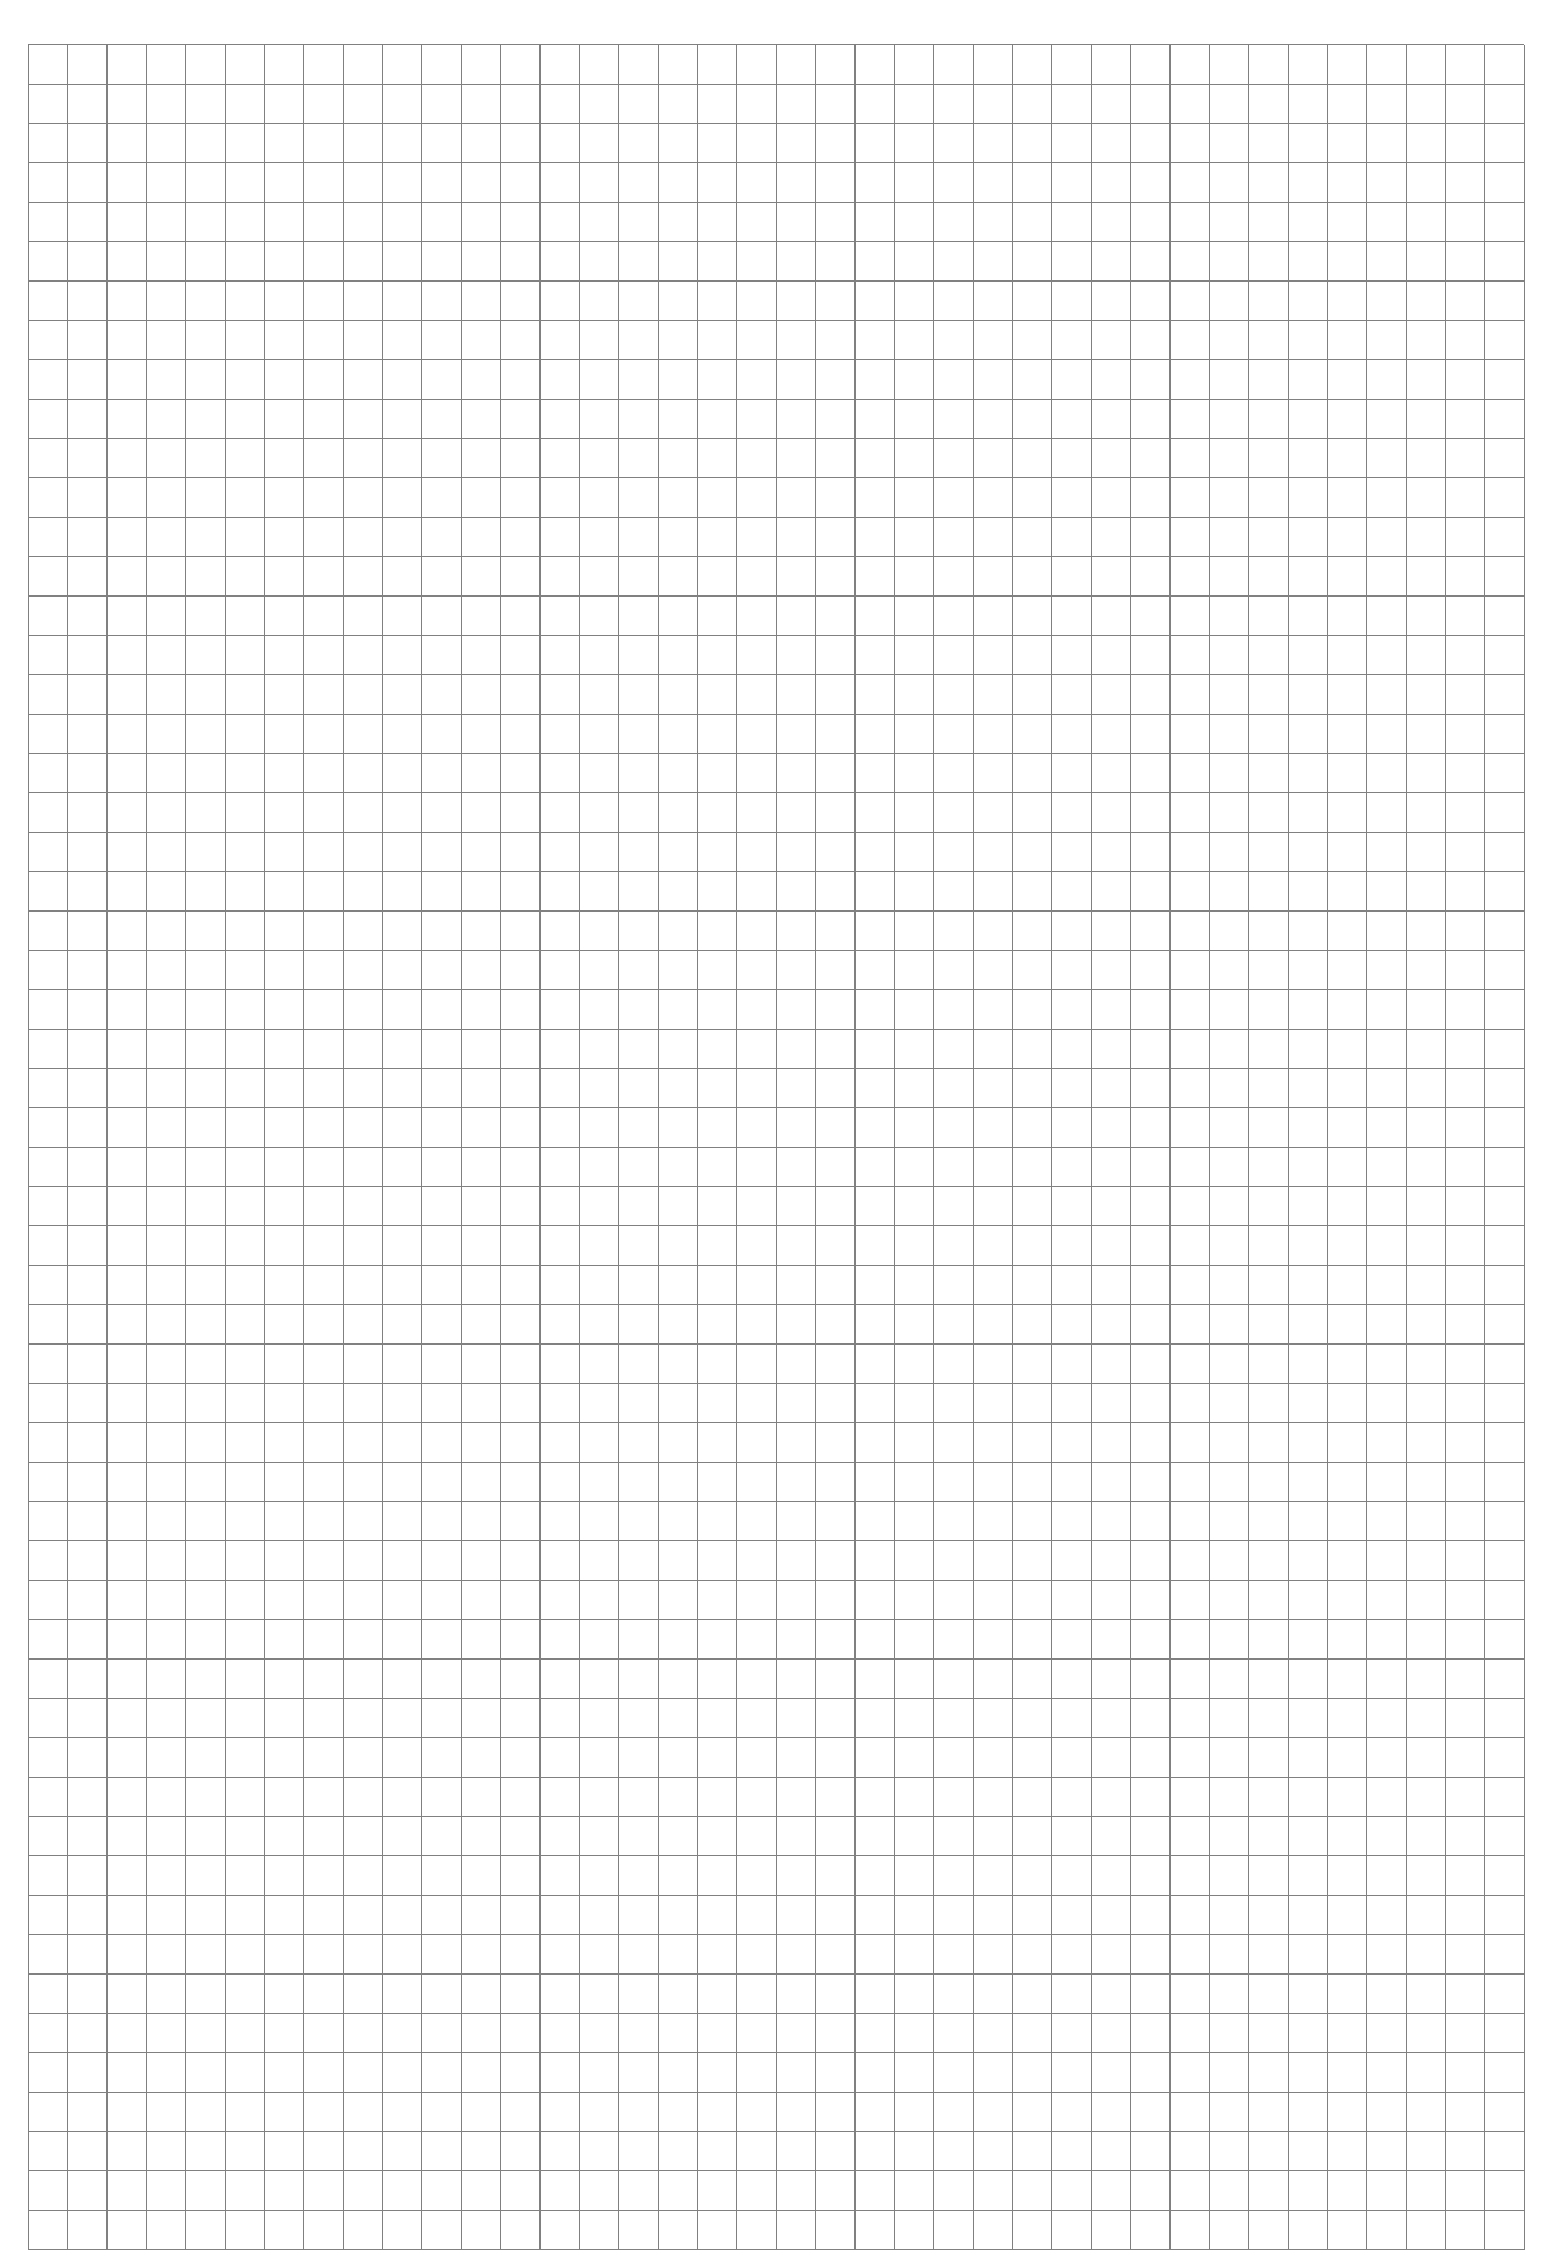
\begin{tikzpicture}
       \draw[step=0.5, gray, thin] (0,0) grid (19, 28.0);
   \end{tikzpicture}
\end{center}
%\newpage
%\begin{center}
%    \begin{tikzpicture}
%        \draw[step=0.5, gray, thin] (0,0) grid (19, 28.0);
%    \end{tikzpicture}
%\end{center}
%\newpage
%\begin{center}
%    \begin{tikzpicture}
%        \draw[step=0.5, gray, thin] (0,0) grid (19, 28.0);
%    \end{tikzpicture}
%\end{center}
%\newpage
%\begin{center}
%    \begin{tikzpicture}
%        \draw[step=0.5, gray, thin] (0,0) grid (19, 28.0);
%    \end{tikzpicture}
%\end{center}

\end{document}

